\documentclass{superfri}
\usepackage{polski}
\usepackage[utf8]{inputenc}
\usepackage{graphicx}

\usepackage{listings}
\usepackage{color}
\definecolor{mygreen}{rgb}{0,0.6,0}
\definecolor{mygray}{rgb}{0.5,0.5,0.5}
\definecolor{mymauve}{rgb}{0.58,0,0.82}
\lstset{ %
  backgroundcolor=\color{white},   % choose the background color; you must add \usepackage{color} or \usepackage{xcolor}; should come as last argument
  basicstyle=\footnotesize,        % the size of the fonts that are used for the code
  breakatwhitespace=false,         % sets if automatic breaks should only happen at whitespace
  breaklines=true,                 % sets automatic line breaking
  captionpos=b,                    % sets the caption-position to bottom
  commentstyle=\color{mygreen},    % comment style
  deletekeywords={...},            % if you want to delete keywords from the given language
  escapeinside={\%*}{*)},          % if you want to add LaTeX within your code
  extendedchars=true,              % lets you use non-ASCII characters; for 8-bits encodings only, does not work with UTF-8
  frame=single,	                   % adds a frame around the code
  keepspaces=true,                 % keeps spaces in text, useful for keeping indentation of code (possibly needs columns=flexible)
  keywordstyle=\color{blue},       % keyword style
  language=Octave,                 % the language of the code
  morekeywords={*,...},           % if you want to add more keywords to the set
  numbers=left,                    % where to put the line-numbers; possible values are (none, left, right)
  numbersep=5pt,                   % how far the line-numbers are from the code
  numberstyle=\tiny\color{mygray}, % the style that is used for the line-numbers
  rulecolor=\color{black},         % if not set, the frame-color may be changed on line-breaks within not-black text (e.g. comments (green here))
  showspaces=false,                % show spaces everywhere adding particular underscores; it overrides 'showstringspaces'
  showstringspaces=false,          % underline spaces within strings only
  showtabs=false,                  % show tabs within strings adding particular underscores
  stepnumber=2,                    % the step between two line-numbers. If it's 1, each line will be numbered
  stringstyle=\color{mymauve},     % string literal style
  tabsize=2,	                   % sets default tabsize to 2 spaces
  title=\lstname                   % show the filename of files included with \lstinputlisting; also try caption instead of title
}


% ------------

%\bibliographystyle{plain}
\begin{document}

\classify{Praca dyplomowa magisterska}
\author{Marcin Skwarek\footnote{\label{susu}Politechnika Warszawska, Wydział Elektroniki i Technik Informacyjnych, Instytut Telekomunikacji}}

\title{Raport z prac w ramach PDMGR}

\maketitle{}

\begin{abstract}%
Abstract: TBA

\keywords{PDMGR, WUT, WEiTI, IT, malware domain, DNS, AXFR}

\end{abstract}

% -----------------------------------------------------------------------
\pagestyle{plain}
\LaTeX.
\section*{Wstęp}
\label{sec:intro}
Głównym tematem pracowni dyplomowej magisterskiej w semestrze 16Z było zagadnienie podatności serwerów DNS ze szczególnym uwzględnieniem wykorzystania zapytań AXFR. Problemem postawionym w tym semestrze było zaprojektowanie i uruchomienie systemu umożliwiającego analizę tej podatności oraz sporządzenie raportu technicznego z przeprowadzonych prac. 

\section{Wstęp teoretyczny}

DNS Zone Transfer Protocol (AXFR) został opisany w RFC 5936\cite{RFC5936}. Mechanizm został zaprojektowany w celu umożliwienia przesyłania informacji pomiędzy serwerami systemu DNS. Typową sytuacją kiedy pomocne jest wykorzystanie protokołu AXFR jest edycja danych na jednym z kilku serwerów DNS i wykorzystanie protokołu aby przepropagować zmiany na kolejne maszyny.

Zapytania AXFR bywają oczywiście wykorzystywane przez cyberprzestępców, którzy chcą wykraść dane przechowywane w plikach konfiguracyjnych serwerów. Wysyłają oni zapytania licząc na błąd przy konfiguracji serwera DNS, który zwróci informacje o domenach obsługiwanych przez daną maszynę. Jeszcze kilka lat temu takie działanie niemal zawsze kończyło się pozyskaniem danych, jednak administratorzy zwracają na to większą uwagę i duża liczba serwerów jest odporna na tę podatność.

Przykładem wykorzystania opisywanej podatności jest atak na serwery firmy Western Digital opisany w SecurityWeek \cite{wd} w kwietniu poprzedniego roku. Okazało się, że jeden z serwerów DNS obsługujących domenę wd2go.com był źle skonfigurowany i odpowiadał na zapytania AXFR, co pozwoliło uzyskać dostęp do niemal 6 milionów wpisów w tym ponad milion unikatowych adresów IP, które należały do klientów koncernu WesterDigital.

AXFR sam w sobie nie jest krytyczną luką w systemach, niemniej jednak może dawać atakującemu dużą ilość informacji na temat potencjalnej ofiary. Jak przestawiono w przytoczonym wcześniej artykule \cite{wd} ewentualnym problemem, który może wyniknąć z przeprowadzonego ataku może być wygenerowanie listy adresów IP klientów. Jeśli w oprogramowaniu urządzenia wykryto by błąd, to atakujący dokładnie wie, czyje dane może starać się wykraść, a nawet ma dokładny adres urządzeń, które mogą posiadać tę lukę.
\section{Podobne prace}

Podczas szukania informacji na temat zagadnienia zapytań AXFR w kontekście cyberbezpieczeństwa natrafiono na projekt wykorzystujący tę samą podatność, jednak nastawiony na inne cele. Chodzi mianowicie o axfr-tools\cite{axfrtools} jednak autorzy projektu większy nacisk kładą na konkretną domenę i zbieranie historycznych zapisów, niż na analizowanie ogólnego trendu. Autorzy nie mieli również narzuconych ograniczeń czasowych skanowania, dlatego mogli pozwolić sobie na używanie narzędzi dostępnych w systemie linux (grep, sed, powłoka bash, produkcyjna wersja dig\'a) oraz na jednowątkowe generowanie zapytań. Warto dodać, że projekt był rozwijany w podobnym czasie co niniejsza praca magisterska, co może dowodzić temu, że temat cieszy się zainteresowaniem różnych osób (w tym przypadku pentesterów).


\section{Zaprojektowany system}

Podstawowym kryterium przy projektowaniu opisywanego systemu była jego wydajność. W założeniu powinien on skanować jak najwięcej domen w możliwie najkrótszym czasie. Nałożone ograniczenia wynikały z kilku istotnych przyczyn. 

Pierwszą była ograniczona dostępność odpowiednio wydajnej maszyny. Dzięki uprzejmości dra Macieja Korczyńskiego z TU Delft otrzymaliśmy możliwość skorzystania z wydajnego serwera, jednak mogliśmy z niego skorzystać tylko przez krótki czas. Czas ten wynosił około 5 dni, gdzie w stosunku do ogromu danych jakie należało przeanalizować okazało się to niewystarczające. Niemniej jednak została przeprowadzona pewna część całego skanowania, dzięki czemu pozyskaliśmy informacje umożliwiające dalsze prace w zakresie ich analizy. 

Kolejne ograniczenie odnosi się już do samej istoty systemu DNS. Jeżeli skanowanie opisane w niniejszym raporcie byłoby zbyt długo rozciągnięte w czasie, to moglibyśmy wyciągnąć niepoprawne wnioski. Chodzi tu głównie o zmiany, które można określić jako ogólne, po prostu zachodzące w sieci. Mamy tu na myśli choćby dynamicznie przydzielane IP prze różnych dostawców internetu. Jako przykład może posłużyć bardzo prosty scenariusz opisany poniżej:
\begin{enumerate}
    \item Odpytujemy domenę x.
    \item W odpowiedzi domeny otrzymujemy adres a.b.c.d .
    \item Skanowanie innych domen trwa bardzo długo.
    \item Adres a.b.c.d zostaje przydzielony do domeny y.
    \item Skanujemy domenę y, otrzymujemy ten sam adres, co dla domeny x.
\end{enumerate}
Na podstawie powyższego scenariusza możemy wyciągnąć bardzo pochopny wniosek, że domeny x i y mają choćby wspólny serwer. Niekoniecznie musi to być prawda, ponieważ jak przestawiono, przyczyna może leżeć w sposobie przydzielania adresów przez usługodawcę. 

Oczywiście w idealnym przypadku, najlepiej byłoby zrobić skanowanie całego zbioru danych wejściowych w jednym, ustalonym stanie sieci, jednak biorąc pod uwagę akademickie możliwości, nie było to zbyt oczywiste do wykonania.

Ograniczenia nałożone na przedstawiony problem wymagały użycia odpowiednich narzędzi. W przedstawionym przypadku zdecydowano na wykorzystanie systemu operacyjnego Linux oraz napisaniu programu wykonującego skanowanie.

Implementacja odpowiedniej logiki trwała relatywnie długo w porównaniu do reszty prac. Dojście do ostatecznej wersji systemu zajęło około dwóch miesięcy. Wpływ miały na to zarówno technologia (język C), zagadnienie programowania sieciowego jak i standardy protokołu DNS. Głównym problemem był brak dobrych bibliotek wspierających protokół DNS. Jeśli już takowe się pojawiały, to głównie w kontekście oferowania translacji nazw domen na adresy IP, nie umożliwiając wysłania zapytania AXFR. 

Kolejną próbą rozwiązania tego problemu było skorzystanie z kodów źródłowych programu dig, który wchodzi w zakres pakietu BIND. Rzeczywiście program wspiera wysyłanie i odbieranie zapytań AXFR. Mimo wszystko, pakiet dotknięty jest typowymi problemami oprogramowania open source. Po pierwsze nie ma spójnej implementacji, różne moduły są napisane w inny sposób co utrudnia czytanie takich źródeł. Po drugie, w momencie podjęcia próby rozszerzenia programu o możliwość parsowania danych wejściowych i odpytywania kolejnych domen w pętli programista może się niezwykle rozczarować. Okazuje się bowiem, że program dig powoduje tzw. ,,wycieki pamięci'', przez co już przy drugiej próbie odpytania domeny w tym samym procesie jest on kończony. Wynikiem prac nad tym problemem jest również raport z programu valgrind wysłany do Internet Systems Consortium informujący o wykrytym problemie z pamięcią. Raport został również dołączony do niniejszej pracy jako załącznik 1.

Niestety podobne problemy pojawiały się przy próbie implementacji sportowanej biblioteki do języka C++. Postanowiono więc poszukać innego rozwiązania, czyli ,,nabudowania'' menadżera, który zarządza kolejnymi procesami.

Ważną zmianą jaką zdecydowano się podjąć, była kompilacja programu dig ze źródeł, z kilkoma poprawkami na potrzeby tego zadania. Ograniczały się one do usunięcia niechcianego wydruku przy prezentacji wyników. Początkowo celem było wydzielenie specjalnego interfejsu w języku C, który bazowałby na implementacji programu dig, jednak z wyżej wymienionych powodów nie było to możliwe. Dlatego zdecydowano się na rozwiązanie pośrednie, a konkretnie usunięcie wszystkich niepotrzebnych informacji z wydruku działania programu dig, skompilowanie i bazowanie na tej wersji aplikacji.  

Opisywany wariant zdecydowano się implementować w Pythonie. Wykorzystano mechanizm tak zwanych wątków programowych, dostępny w tym języku. Każde z zapytań programu dig było uruchamiane jako zupełnie odrębny proces, co zapewniało, że otrzyma on swoje zasoby. W ten sposób możliwe było obejście wycieków pamięci, które zostały zdiagnozowane przy okazji poprzednich prac. Wspomniane podprocesy były uruchamiane współbieżnie dopóki na serwerze występowały wolne zasoby. Niestety, jak się później okazało, i ta implementacja posiadała swoje wady, a główną było wykorzystanie tylko jednego fizycznego procesora. Zostało to zdiagnozowane dopiero na bardzo wydajnym serwerze. Aby nie rozbudowywać niepotrzebnie implementacji, zdecydowano się na uruchamianie kilku odrębnych menadżerów procesów. Zarządzanie menadżerami odbywało się już na poziomie powłoki systemu Linux, głównie przy użyciu skryptów bashowych.

Założono, że przeskanowanych zostanie ponad 3.3 miliarda par domena - serwer autorytatywny. Dane wejściowe zostały podzielone na około 33 tysiące plików, w każdym po 100 tysięcy par do przeskanowania. Jedna iteracja skryptu przygotowanego w Pythonie zakładała przeanalizowanie jednego z 33 tysięcy plików.

Wyniki działania programów zapisywane są do specjalnej struktury plików. Każda iteracja zapisywana była do oddzielnego folderu. Każdy z folderów miał bliźniaczą strukturę. Składał się z pliku, w którym przechowywane były informacje o wyniku skanowania pary:
\begin{itemize}
    \item upłynięcie limitu czasu żądania,
    \item błędna odpowiedź od serwera,
    \item odpowiedź poprawna,
    \item błąd nieznany.
\end{itemize}
Drugim elementem był folder, w którym przechowywano odpowiedzi od serwerów. W folderze z odpowiedziami znajdowały się pliki, których nazwy określały domenę, o której dane przechowują. 


\section{Wyniki}
Pomimo stosunkowo krótkiego działania skanera, udalo zaobserwować się, że wiele domen rzeczywiście odpowiada na zapytania AXFR. Konkretne wyniki zostały zaprezentowane na rysunku \ref{fig:odpowiedzi}. Możemy zauważyc, że w kilku iteracjach było bardo wiele odpowiedzi. Dane wejściowe były uporządkowane według nazw, więc można postawić hipotezę, że o te same domeny odpytywano kilka serwerów autorytatywnych i większośc była rzeczywiście źle skonfigurowana. Innym powodem może byc po prostu czynnik losowy, jednak zastanawiające jest, że trzy iteracje znacznie wyróżniają się na tle innych.


\begin{figure}
    \centering
        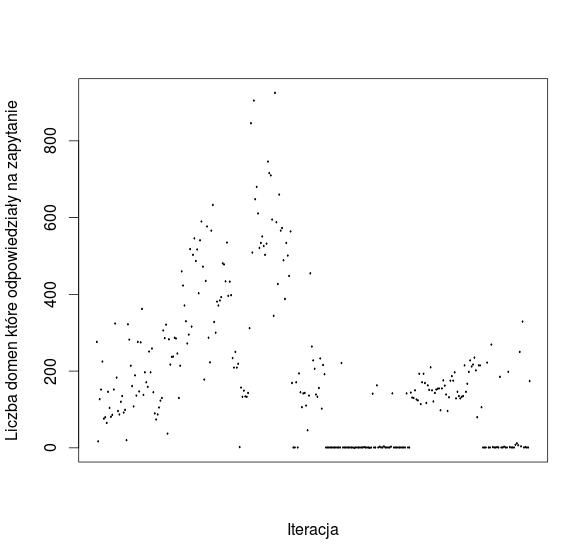
\includegraphics[width=0.8\textwidth]{odpowiedzi.png}
    \caption{ Liczba domen które odpowiedziały na zapytanie AXFR w danej iteracji.} \label{fig:odpowiedzi}
\end{figure}


Innym interesującym zjawiskiem są wpisy TXT\cite{RFC1035}, które zwracają niektóre serwery. Wpis TXT był wprowadzony głównie po to, aby ułatwić ludzie mogli przeczytać informację, która zostanie zawarta w odpowiedzi DNS. Z czasem oczywiście okazało się, że wpis częściej jest używany przez komputery niż ludzi, czego przykład mamy w odpowiedziach.

Pierwsyzm przykładem może być znalezienie reguły SPF\cite{RFC7208}:
\begin{lstlisting}
"v=spf1 ip4:52.72.252.186/13 ip4:52.220.30.76/15 ip4:54.179.130.187/15 ip4:52.95.240.219/20 ip4:54.251.128.33/12 ip4:114.134.29.0/23 ip4:54.169.107.198/15 ip4:46.51.216.57/20 ip4:103.228.178.81/15 ip4:157.119.230.135/14 ip4:103.44.71.16/15 ~all"
\end{lstlisting}

Z wyżej przytoczonej reguły można wywnioskować maszyny o jakich adresach są ,,specjalnie'' traktowane przez serwer. W skrócie, reguły SPF mówią, które z serwerów są upoważnione do wysyłania wiadomości z domeny. Dodatkowo parametr ,,\~all'' (jak na przykładzie powyżej) określa, że wiadomości od serwerów nie spełniających reguły będą odrzucane, lub oznaczane jako spam.

Oprócz opisanego przypadku użycia pola TXT pojawiały się także i inne, jednak nie do końca udało się je rozszyfrować. Niektóre z przytoczonych sposobów wykorzystania tego pola są oczywiście poprawne. Jednym z przykładów użycia jest wklejenie klucza publicznego. Jest to również swego rodzaju zabezpieczenie serwera przed spamem. Przykład poniżej.

\begin{lstlisting}
"v=DKIM1; k=rsa; p=MIIBIjANBgkqhkiG9w0BAQEFAAOCAQ8AMIIBCgKCAQEApt/kMkRxGXbIuiVb4lCYeTQMEOBKTXTUJya8aY659OB0feNIoA070AHq4M7/KKa4u/T/BfLNVNfyaK56S1E7S9o" "HItQUFO5idWKBRAK/VnK0I9FjWMlAMamQItiLmaUWtC4VhB5n0JzgPmutqx4qDo/IVIp97bWm3FDe4ts1zMNODxTTql52hkZ/X91/HrZYrC3qBLAg4rHbgBnJHWny55yt7vkgknyh7MAuN5qZDlN4s" "xrlOTbuJYGOCo2OTR8WteWorDC4qw41CTr273QiB/suVSZODeZD9xNKN6fmoFNCfhwUqXVzAiDVT0RcfNDmM1istoJyoVu56CCuHIJnowIDAQAB"
\end{lstlisting}

Mimo, że wpis ten wydaje się być poprawny, a nawet uzasadnione jest jego użycie, mam pewne obawy co do tego, czy rzeczywiście powinien być zwracany przez zapytanie AXFR.
\section{Podsumowanie}

Podsumowując swoją pracę, chciałbym na pewno krytycznie na nią spojrzeć. Uważam, że zdecydowanie szybciej powinienem dojść do rozwiązania, które zostało ostatecznie wybrane. Zbyt dużo czasu zostało poświęconego na przedwczesną optymalizację. Ponadto, dużym problemem okazało się uruchomienie systemu na wydajniejszej maszynie. Pomimo dołożenia wszelkich starań do tego, aby system trafił już w pełni przetestowany i gotowy do działania nie udało się uniknąć problemów, które skróciły czas działania skanera. Mam tu głównie na myśli niepełne wykorzystanie dostępnych zasobów, które było widoczne dopiero na wydajnym komputerze.

Pomimo napotkanych problemów, myślę, że prace zostały wykonane w dużym stopniu. Z pewnością cieszy fakt, że można szukać ,,spektakularnych'' przypadków wykorzystania podatności AXFR na prawdziwych danych. 

To, co chciałbym zrealizować w najbliższej przyszłości to oczywiście dokładniejsze przestudiowanie zebranych informacji. Na razie skupiono się głównie na analizie wpisów TXT, co widać również w tym dokumencie. Być może nie był to dobry kierunek, jednak te wpisy wydawały się najbardziej intrygujące oraz niepasujące do innych danych umieszczonych w pliku strefy (zone'y ?).

Największą obawę budzi we mnie to, jakie ograniczenia wydajnościowe zostały nałożone na system. Obawiam się, że może być trudne sprostanie wszystkim wymaganiom (a w szczególności czasowi skanowania).

Jeśli chodzi o dalsze prace w zakresie analizy pozyskanych danych, myślę, że należy przeanalizować korelację między serwerami które odpowiedziały na zapytanie dla danej domeny a zapytaniem whois. Innym pomysłem może być zliczenie ile razy pojawia się konkretny adres IP w kontekście odpowiedzi AXFR.




%\cite{Cadez:2000:VNP:347090.347151,Stonebraker:1994:PND:190956.191247}.



\ack{}

\bibliography{bibliografia}
\nocite{*}
\bibliographystyle{plain}


\newpage\section*{Załącznik 1.}
\begin{lstlisting}
==12119== Memcheck, a memory error detector
==12119== Copyright (C) 2002-2013, and GNU GPL'd, by Julian Seward et al.
==12119== Using Valgrind-3.10.1 and LibVEX; rerun with -h for copyright info
==12119== Command: dig pw.edu.pl AXFR
==12119== 

; <<>> DiG 9.2.3 <<>> pw.edu.pl AXFR
;; global options:  printcmd
; Transfer failed.
==12119== 
==12119== HEAP SUMMARY:
==12119==     in use at exit: 240 bytes in 7 blocks
==12119==   total heap usage: 54 allocs, 47 frees, 222,504 bytes allocated
==12119== 
==12119== LEAK SUMMARY:
==12119==    definitely lost: 0 bytes in 0 blocks
==12119==    indirectly lost: 0 bytes in 0 blocks
==12119==      possibly lost: 0 bytes in 0 blocks
==12119==    still reachable: 240 bytes in 7 blocks
==12119==         suppressed: 0 bytes in 0 blocks
==12119== Rerun with --leak-check=full to see details of leaked memory
==12119== 
==12119== For counts of detected and suppressed errors, rerun with: -v
==12119== ERROR SUMMARY: 0 errors from 0 contexts (suppressed: 0 from 0)
\end{lstlisting}


\received{Styczeń 12, 2017}

\end{document}


